% =====================================================================
%  CricketMind -- Architecture Draft v3
%  Verified Claims over Real Evidence
%
%  Revision notes vs. v2:
%    * Subject-keyed claim contract: agents emit claim tuples, never
%      typed numbers; the Faith Check re-queries the engines per tuple.
%    * Uncertainty-faithful verification: predictive and comparative
%      claims carry the engine's interval, and their wording must fit it.
%      N9's interval now includes estimation uncertainty, not only
%      Monte Carlo error.
%    * Claim-type registry, checked when the graph is built: no agent
%      may assert a kind of claim that no engine computes.
%    * N8 gains three modules (venue profile, bowling workload, DRS
%      reviews); N9 gains Tier 2 matchup counterfactuals with calibration.
%    * Real evidence: Cricsheet ball-by-ball data, player attributes, and
%      an offline commentary-to-shot bridge.
%    * N2b pose estimator: posture is measured, no longer looked up.
%    * Roster: Bowling Performance added; Compliance reframed as Match
%      Officials; Sponsorship merged into Content Production.
%
%  Status: design. No v3 component has been built or measured.
%  Compile with: pdflatex CricketMind_Architecture_v3.tex   (run twice)
% =====================================================================
\documentclass[11pt,a4paper]{article}

\usepackage[margin=2cm]{geometry}
\usepackage[T1]{fontenc}
\usepackage[utf8]{inputenc}
\usepackage{lmodern}
\usepackage{booktabs}
\usepackage{array}
\usepackage{xcolor}
\usepackage{amsmath}
\usepackage{enumitem}
\usepackage{float}
\usepackage{capt-of}
\usepackage[font=small,labelfont=bf,hypcap=false]{caption}
\usepackage{tikz}
\usetikzlibrary{shapes.geometric,arrows.meta,positioning,calc,fit,backgrounds}
\usepackage[hidelinks]{hyperref}
\def\UrlBreaks{\do\/\do-\do\_}
\setlength{\emergencystretch}{1.5em}

% ---------------------------------------------------------------- colours
\definecolor{encblue}{RGB}{31,58,110}      % vision / text encoding
\definecolor{fuseteal}{RGB}{17,110,110}    % multimodal fusion
\definecolor{retbrown}{RGB}{124,76,38}     % retrieval
\definecolor{svcorange}{RGB}{176,90,20}    % sanctioned engines
\definecolor{routeviolet}{RGB}{88,48,132}  % supervisor / router
\definecolor{agentgreen}{RGB}{27,94,58}    % stakeholder agents
\definecolor{gatered}{RGB}{170,30,40}      % confidence gate
\definecolor{gatepurple}{RGB}{112,44,132}  % faithfulness gate
\definecolor{dbtan}{RGB}{222,196,160}      % databases
\definecolor{outgrey}{RGB}{45,45,50}       % final output
\definecolor{gateslate}{RGB}{72,88,104}    % entry branch
\definecolor{newgold}{RGB}{214,160,20}     % new or changed in v3

% ---------------------------------------------------------------- styles
\tikzset{
  base/.style   = {draw, rounded corners=2pt, align=center, font=\small,
                   minimum width=2.9cm, minimum height=1.1cm, inner sep=3pt,
                   line width=0.7pt},
  enc/.style    = {base, fill=encblue,     text=white, draw=encblue!55!black},
  fuse/.style   = {base, fill=fuseteal,    text=white, draw=fuseteal!55!black},
  ret/.style    = {base, fill=retbrown,    text=white, draw=retbrown!55!black},
  svc/.style    = {base, fill=svcorange,   text=white, draw=svcorange!55!black},
  route/.style  = {base, fill=routeviolet, text=white, draw=routeviolet!55!black},
  agent/.style  = {base, fill=agentgreen,  text=white, draw=agentgreen!55!black,
                   minimum width=2.7cm, minimum height=1.2cm, font=\footnotesize},
  outnode/.style    = {base, fill=outgrey,     text=white, draw=black},
  gate/.style   = {draw, diamond, aspect=2.0, align=center,
                   font=\footnotesize\bfseries, inner sep=2pt, line width=0.7pt},
  confgate/.style  = {gate, fill=gatered,    text=white, draw=gatered!55!black},
  faithgate/.style = {gate, fill=gatepurple, text=white, draw=gatepurple!55!black},
  entrygate/.style = {gate, fill=gateslate,  text=white, draw=gateslate!55!black},
  db/.style     = {draw, cylinder, shape border rotate=90, aspect=0.28,
                   fill=dbtan, align=center, font=\scriptsize,
                   minimum width=1.8cm, minimum height=1.0cm, line width=0.7pt},
  flow/.style   = {-{Stealth[length=2.4mm]}, line width=0.9pt, draw=black!72},
  bus/.style    = {line width=0.9pt, draw=black!72},
  redloop/.style   = {-{Stealth[length=2.4mm]}, line width=0.9pt,
                   draw=gatered, dashed, dash pattern=on 4pt off 2.5pt},
  redbus/.style = {line width=0.9pt, draw=gatered, dashed,
                   dash pattern=on 4pt off 2.5pt},
  yield/.style  = {-{Stealth[length=2.2mm]}, line width=0.8pt,
                   draw=agentgreen!85, dashed, dash pattern=on 3pt off 2pt},
  ybus/.style   = {line width=0.8pt, draw=agentgreen!85, dashed,
                   dash pattern=on 3pt off 2pt},
  static/.style = {-{Stealth[length=2.2mm]}, line width=0.8pt, draw=black!55,
                   dash pattern=on 1.5pt off 1.5pt},
  withhold/.style = {-{Stealth[length=2.2mm]}, line width=0.8pt,
                   draw=black!45, dashed, dash pattern=on 3pt off 2pt},
  elab/.style   = {font=\scriptsize\itshape, inner sep=1.5pt, fill=white},
  % --- v3 additions
  v3/.style     = {draw=newgold, line width=1.8pt},
  badge/.style  = {circle, draw=#1, line width=1pt, fill=white, text=#1,
                   font=\scriptsize\bfseries, inner sep=0pt, minimum size=0.5cm},
  registry/.style = {draw=black!60, dashed, rounded corners=2pt, fill=black!6,
                   align=center, font=\scriptsize, text width=2.2cm,
                   minimum height=1.0cm, inner sep=3pt},
  off/.style    = {base, fill=retbrown!10, text=black, draw=retbrown,
                   minimum width=3.2cm},
  chk/.style    = {base, fill=gatepurple!10, text=black, draw=gatepurple,
                   minimum width=2.6cm},
}

\title{\textbf{CricketMind}\\[0.3em]
       \large Verified Claims over Real Evidence\\[0.2em]
       \normalsize Thesis Architecture Draft --- Version 3}
\author{}
\date{}

\begin{document}
\maketitle
\thispagestyle{empty}

\begin{center}
\fbox{\parbox{0.92\textwidth}{\small
\textbf{Status.} This is a design. No v3 component has been built or measured.
Every number in this document is a design parameter, a figure cited from the
literature, or an illustrative computation on the synthetic corpus of the v2
reference implementation, and is labelled as such. The accuracy of the
perception front end is evaluated separately and is not reported here.}}
\end{center}

% =====================================================================
\section{What Changes in Version 3, and Why}

Version~2 established the control flow: two entry paths, two bounded correction
loops, twelve stakeholder agents, and a Faith Check that compares every cited
figure against two sanctioned engines. Its evaluation also exposed four gaps,
and Version~3 is organised around closing them.

\begin{enumerate}[leftmargin=1.6em]
\item \textbf{The gate verifies values, not claims.} It rejected fabricated
  citations but passed a correct figure attached to the wrong subject and a
  figure stated without a citation. The conclusion of that evaluation already
  names a subject-keyed citation contract as a requirement for language-model
  agents.
\item \textbf{Four agents assert claims that no engine computes.} The Stadium
  agent says the surface ``is holding pace'' while citing only a ball count;
  the Compliance agent reports ``no eligibility flags'' with no compliance data;
  the Injury agent says a workload ``sits inside the weekly threshold'' without
  computing a workload, and counts balls \emph{faced}; the Sponsorship agent
  names the ``most replayed shot'' with no replay data. Each passes the gate,
  because the number it cites is correct. Three more agents make salary,
  valuation or selection recommendations with no market data behind them.
\item \textbf{Predictive claims are verified as if they were facts.} N9 already
  computes a 95\% interval, but no agent cites it and the gate never reads it.
  Worse, that interval measures only Monte Carlo error
  (Section~\ref{sec:uncert}).
\item \textbf{The evidence is synthetic, and real ball-by-ball data has no shot
  type.} Cricsheet records every delivery but not which stroke was played, so
  the shot the video identifies has nowhere to land.
\end{enumerate}

\noindent Table~\ref{tab:changes} lists the changes. The principle of v2 is kept
and sharpened: numbers come only from sanctioned sources, and now every
\emph{kind of claim} must come from one too.

\begin{center}
\footnotesize
\renewcommand{\arraystretch}{1.25}
\begin{tabular}{@{}>{\raggedright\arraybackslash}p{0.4cm}
                  >{\raggedright\arraybackslash}p{4.4cm}
                  >{\raggedright\arraybackslash}p{6.6cm}
                  >{\raggedright\arraybackslash}p{3.6cm}@{}}
\toprule
\textbf{\#} & \textbf{Change} & \textbf{Motivation} & \textbf{Where} \\
\midrule
1 & Subject-keyed claim contract & Gate blind to subject swaps and uncited figures (gap 1) & All agents; Faith Check C1, C2, C5, C6 \\
2 & Uncertainty-faithful verification & Interval computed but unused; Monte Carlo error only (gap 3) & N9; Faith Check C3, C4 \\
3 & Engines behind hollow agents, and a claim-type registry & Claims with no engine behind them (gap 2) & N8 modules M2--M4; registry; N11f, N11i, N11k \\
4 & Real evidence, and N9 Tier~2 matchups with calibration & Synthetic corpus (gap 4) & Delivery DB; N7a, N7b; N8 M1; N9 T2 \\
5 & Commentary-to-shot bridge & No shot type in ball-by-ball data (gap 4) & Offline pipeline O3 \\
6 & Measured posture from pose estimation & Posture was a per-shot lookup constant & N2b; N6 \\
R & Roster: Bowling Performance added; Compliance $\rightarrow$ Match Officials; Sponsorship merged into Content Production & No bowler-side agent; no public data can back compliance or sponsorship claims & N11g, N11h, N11i \\
\bottomrule
\end{tabular}
\captionof{table}{Changes from Version~2. Node letters are kept, so code
identifiers map one-to-one; N11g and N11i change role.}
\label{tab:changes}
\end{center}

% =====================================================================
\section{Design Invariants}
\label{sec:invariants}

Version~3 is defined by six invariants. Every later section is an
implementation of one of them.

\begin{description}[leftmargin=1.2em,style=nextline,itemsep=2pt]
\item[I1 --- Numeric authority.] Only three sources may produce a number:
  N6 (\emph{measured} from the clip), N8 (\emph{descriptive}, counted from
  history) and N9 (\emph{predictive}, simulated). There are still two engines;
  N6 is a measurement, as it already was in v2. N9 remains code and never
  becomes a language-model call.
\item[I2 --- No hollow claims.] Every claim type an agent may assert resolves to
  a metric of one sanctioned source. This is checked when the graph is built,
  so a template that asserts an unsupported kind of claim cannot be deployed.
\item[I3 --- Agents never type numbers.] Agents write prose that references
  claim identifiers. A deterministic renderer inserts the verified values.
\item[I4 --- Uncertainty travels with the claim.] Predictive and comparative
  claims carry their interval, and their wording must be consistent with it.
\item[I5 --- No measurement without a clip.] A text-only query can never carry a
  measured claim; the posture fields are absent, not defaulted.
\item[I6 --- Bounded cost.] Every loop is bounded (at most two retries, two
  regenerations and four active agents), so worst-case cost stays closed-form.
\end{description}

% =====================================================================
\clearpage
\section{System Architecture Diagram}

\begin{center}
\resizebox{!}{0.76\textheight}{%
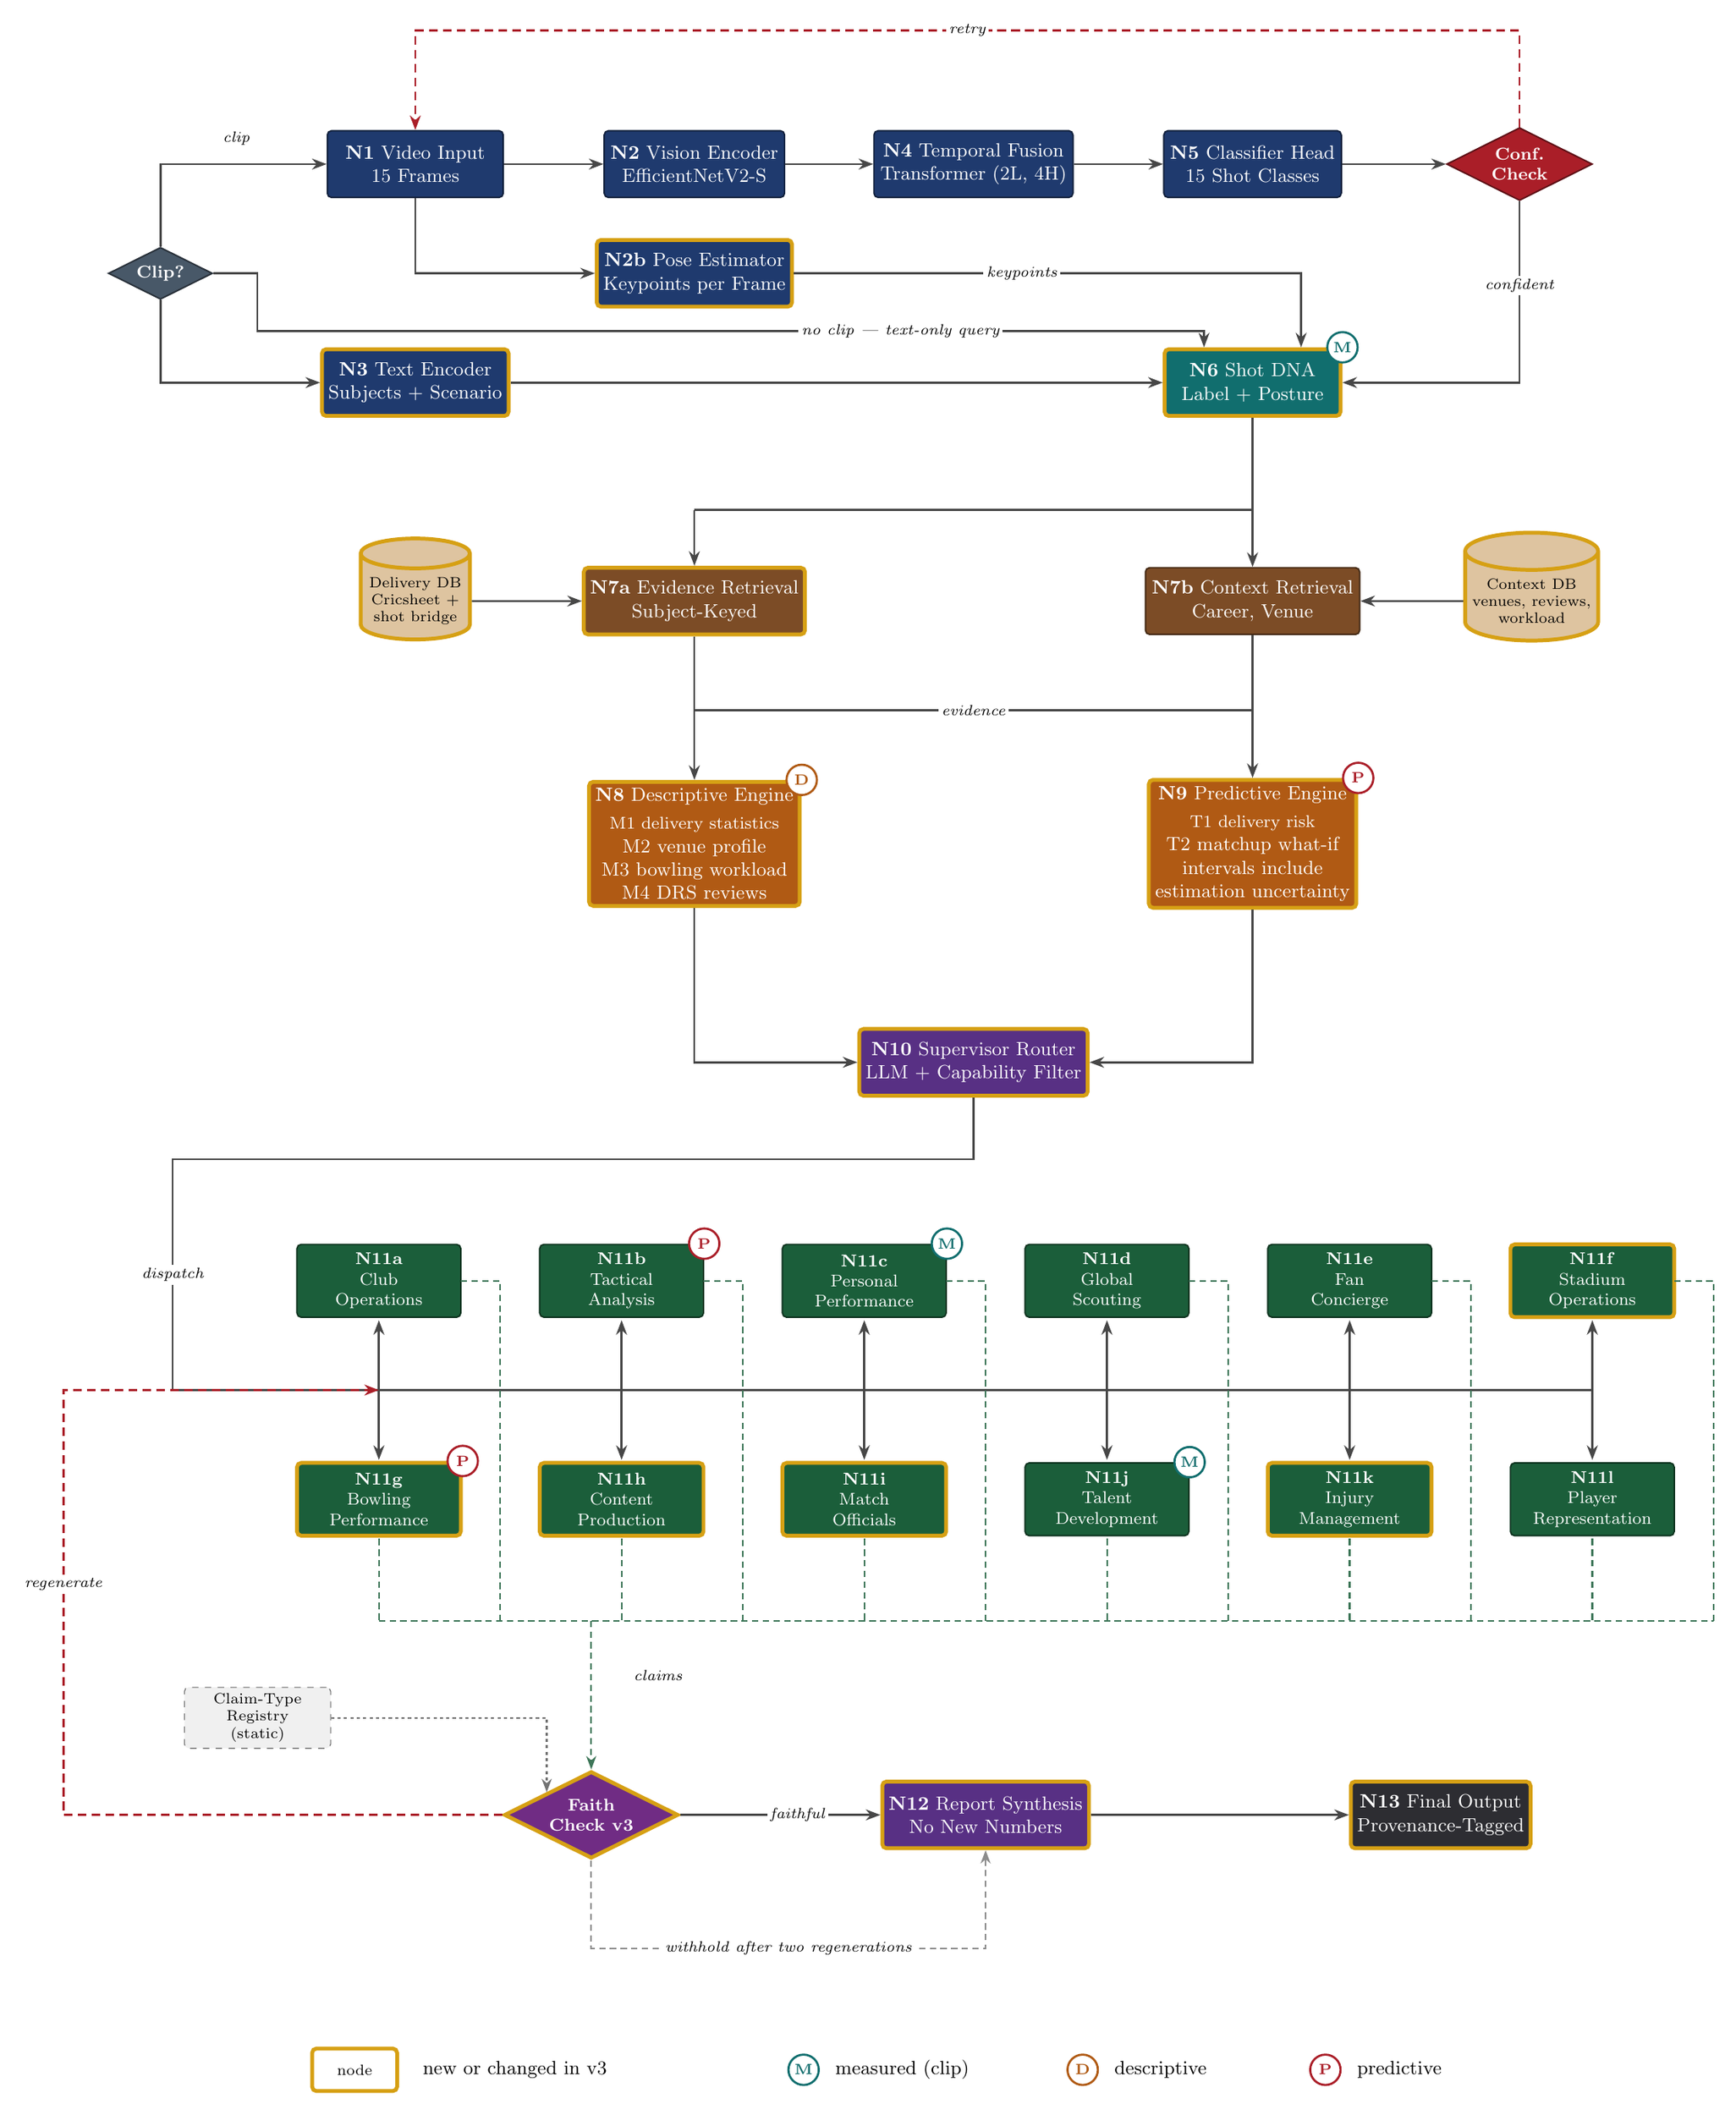
\begin{tikzpicture}

% ============================================ 0. entry branch
\node[entrygate] (entry) at (-2.6,-1.8) {Clip?};

% ============================================ A. encoding chain
\node[enc] (n1)   at (1.6,0)    {\textbf{N1} Video Input\\15 Frames};
\node[enc] (n2)   at (6.2,0)    {\textbf{N2} Vision Encoder\\EfficientNetV2-S};
\node[enc] (n4)   at (10.8,0)   {\textbf{N4} Temporal Fusion\\Transformer (2L, 4H)};
\node[enc] (n5)   at (15.4,0)   {\textbf{N5} Classifier Head\\15 Shot Classes};
\node[confgate] (conf) at (19.8,0) {Conf.\\Check};

% ============================================ A'. pose branch (new)
\node[enc, v3] (n2b) at (6.2,-1.8) {\textbf{N2b} Pose Estimator\\Keypoints per Frame};

% ============================================ B. text branch + grounding
\node[enc, v3]  (n3) at (1.6,-3.6)  {\textbf{N3} Text Encoder\\Subjects + Scenario};
\node[fuse, v3] (n6) at (15.4,-3.6) {\textbf{N6} Shot DNA\\Label + Posture};

% ============================================ C. evidence and retrieval
\node[db, v3]  (db1) at (1.6,-7.2)  {Delivery DB\\Cricsheet +\\shot bridge};
\node[ret, v3] (n7a) at (6.2,-7.2)  {\textbf{N7a} Evidence Retrieval\\Subject-Keyed};
\node[ret]     (n7b) at (15.4,-7.2) {\textbf{N7b} Context Retrieval\\Career, Venue};
\node[db, v3]  (db2) at (20.0,-7.2) {Context DB\\venues, reviews,\\workload};

% ============================================ D. sanctioned engines
\node[svc, v3] (n8) at (6.2,-11.2)
  {\textbf{N8} Descriptive Engine\\[2pt]\footnotesize M1 delivery statistics\\
   M2 venue profile\\ M3 bowling workload\\ M4 DRS reviews};
\node[svc, v3] (n9) at (15.4,-11.2)
  {\textbf{N9} Predictive Engine\\[2pt]\footnotesize T1 delivery risk\\
   T2 matchup what-if\\ intervals include\\ estimation uncertainty};

% ============================================ E. supervisor router
\node[route, v3] (n10) at (10.8,-14.8) {\textbf{N10} Supervisor Router\\LLM + Capability Filter};

% ============================================ F. twelve stakeholder agents
% Written out explicitly rather than with \foreach: a "\\" inside a
% \foreach value list is a known pgffor failure point.
\node[agent]     (ag1)  at (1,-18.4)  {\textbf{N11a}\\Club\\Operations};
\node[agent]     (ag2)  at (5,-18.4)  {\textbf{N11b}\\Tactical\\Analysis};
\node[agent]     (ag3)  at (9,-18.4)  {\textbf{N11c}\\Personal\\Performance};
\node[agent]     (ag4)  at (13,-18.4) {\textbf{N11d}\\Global\\Scouting};
\node[agent]     (ag5)  at (17,-18.4) {\textbf{N11e}\\Fan\\Concierge};
\node[agent, v3] (ag6)  at (21,-18.4) {\textbf{N11f}\\Stadium\\Operations};

\node[agent, v3] (ag7)  at (1,-22.0)  {\textbf{N11g}\\Bowling\\Performance};
\node[agent, v3] (ag8)  at (5,-22.0)  {\textbf{N11h}\\Content\\Production};
\node[agent, v3] (ag9)  at (9,-22.0)  {\textbf{N11i}\\Match\\Officials};
\node[agent]     (ag10) at (13,-22.0) {\textbf{N11j}\\Talent\\Development};
\node[agent, v3] (ag11) at (17,-22.0) {\textbf{N11k}\\Injury\\Management};
\node[agent]     (ag12) at (21,-22.0) {\textbf{N11l}\\Player\\Representation};

% ============================================ G. verification and synthesis
\node[registry] (reg) at (-1.0,-25.6) {Claim-Type\\Registry\\(static)};
\node[faithgate, v3] (faith) at (4.5,-27.2) {Faith\\Check v3};
\node[route, v3] (n12) at (11,-27.2)   {\textbf{N12} Report Synthesis\\No New Numbers};
\node[outnode, v3] (n13) at (18.5,-27.2) {\textbf{N13} Final Output\\Provenance-Tagged};

% ============================================ provenance badges
\node[badge=fuseteal]  at (n6.north east) {M};
\node[badge=svcorange] at (n8.north east) {D};
\node[badge=gatered]   at (n9.north east) {P};
\node[badge=gatered]   at (ag2.north east) {P};
\node[badge=gatered]   at (ag7.north east) {P};
\node[badge=fuseteal]  at (ag3.north east) {M};
\node[badge=fuseteal]  at (ag10.north east) {M};

% ==================================================================
%                              EDGES
% ==================================================================

% ---- entry branch.  The text-only bypass runs in its own lane at y=-2.75,
%      between the pose row and the text row, and enters N6 from the north.
\draw[flow] (entry.north) -- (-2.6,0) -- (n1.west);
\node[elab] at (-1.35,0.42) {clip};
\draw[flow] (entry.south) -- (-2.6,-3.6) -- (n3.west);
\draw[flow] (entry.east) -- (-1.0,-1.8) -- (-1.0,-2.75) -- (14.6,-2.75)
            -- (14.6,0 |- n6.north);
\node[elab] at (9.6,-2.75) {no clip --- text-only query};

% ---- encoding chain
\draw[flow] (n1) -- (n2);
\draw[flow] (n2) -- (n4);
\draw[flow] (n4) -- (n5);
\draw[flow] (n5) -- (conf);

% ---- pose branch: same frames, parallel to the encoder chain
\draw[flow] (n1.south) -- (1.6,-1.8) -- (n2b.west);
\draw[flow] (n2b.east) -- (16.2,-1.8) -- (16.2,0 |- n6.north);
\node[elab] at (11.6,-1.8) {keypoints};

% ---- retry loop
\draw[redloop] (conf.north) -- (19.8,2.2) -- (1.6,2.2) -- (n1.north);
\node[elab] at (10.7,2.2) {retry};

% ---- confident -> Shot DNA
\draw[flow] (conf.south) -- (19.8,-3.6) -- (n6.east);
\node[elab] at (19.8,-2.0) {confident};

% ---- text encoder -> Shot DNA
\draw[flow] (n3.east) -- (n6.west);

% ---- Shot DNA -> both retrievers
\draw[bus]  (n6.south) -- (15.4,-5.7);
\draw[bus]  (6.2,-5.7) -- (15.4,-5.7);
\draw[flow] (6.2,-5.7)  -- (n7a.north);
\draw[flow] (15.4,-5.7) -- (n7b.north);

% ---- databases -> retrievers
\draw[flow] (db1) -- (n7a);
\draw[flow] (db2) -- (n7b);

% ---- retrievers -> engines: one evidence bus, both engines read it
\draw[bus]  (n7a.south) -- (6.2,-9.0);
\draw[bus]  (n7b.south) -- (15.4,-9.0);
\draw[bus]  (6.2,-9.0) -- (15.4,-9.0);
\draw[flow] (6.2,-9.0)  -- (n8.north);
\draw[flow] (15.4,-9.0) -- (n9.north);
\node[elab] at (10.8,-9.0) {evidence};

% ---- engines -> router
\draw[flow] (n8.south) -- (6.2,-14.8)  -- (n10.west);
\draw[flow] (n9.south) -- (15.4,-14.8) -- (n10.east);

% ---- router -> dispatch bus
\draw[bus] (n10.south) -- (10.8,-16.4) -- (-2.4,-16.4) -- (-2.4,-20.2) -- (1,-20.2);
\draw[bus] (1,-20.2) -- (21,-20.2);
\node[elab] at (-2.4,-18.3) {dispatch};

% ---- dispatch bus -> each agent
\draw[flow] (1,-20.2)  -- (1,-19.05);
\draw[flow] (5,-20.2)  -- (5,-19.05);
\draw[flow] (9,-20.2)  -- (9,-19.05);
\draw[flow] (13,-20.2) -- (13,-19.05);
\draw[flow] (17,-20.2) -- (17,-19.05);
\draw[flow] (21,-20.2) -- (21,-19.05);

\draw[flow] (1,-20.2)  -- (1,-21.35);
\draw[flow] (5,-20.2)  -- (5,-21.35);
\draw[flow] (9,-20.2)  -- (9,-21.35);
\draw[flow] (13,-20.2) -- (13,-21.35);
\draw[flow] (17,-20.2) -- (17,-21.35);
\draw[flow] (21,-20.2) -- (21,-21.35);

% ---- collection bus (green dashed) below row 2
\draw[ybus] (1,-24.0) -- (23,-24.0);

\draw[ybus] (1,-22.65)  -- (1,-24.0);
\draw[ybus] (5,-22.65)  -- (5,-24.0);
\draw[ybus] (9,-22.65)  -- (9,-24.0);
\draw[ybus] (13,-22.65) -- (13,-24.0);
\draw[ybus] (17,-22.65) -- (17,-24.0);
\draw[ybus] (21,-22.65) -- (21,-24.0);

\draw[ybus] (2.35,-18.4)  -- (3,-18.4)  -- (3,-24.0);
\draw[ybus] (6.35,-18.4)  -- (7,-18.4)  -- (7,-24.0);
\draw[ybus] (10.35,-18.4) -- (11,-18.4) -- (11,-24.0);
\draw[ybus] (14.35,-18.4) -- (15,-18.4) -- (15,-24.0);
\draw[ybus] (18.35,-18.4) -- (19,-18.4) -- (19,-24.0);
\draw[ybus] (22.35,-18.4) -- (23,-18.4) -- (23,-24.0);

% ---- claims -> Faith Check; the registry defines what C1 accepts
\draw[yield] (4.5,-24.0) -- (faith.north);
\node[elab] at (5.6,-24.9) {claims};
\draw[static] (reg.east) -- (reg.east -| faith.north west) -- (faith.north west);

% ---- faith check -> synthesis -> output
\draw[flow] (faith.east) -- (n12.west);
\node[elab] at (7.9,-27.2) {faithful};
\draw[flow] (n12.east) -- (n13.west);

% ---- regenerate loop: back to the dispatch bus, failing agents only
\draw[redloop] (faith.west) -- (-4.2,-27.2) -- (-4.2,-20.2) -- (1,-20.2);
\node[elab] at (-4.2,-23.4) {regenerate};

% ---- withhold path: budget spent, the finding is listed but not used
\draw[withhold] (faith.south) -- (4.5,-29.4) -- (11,-29.4) -- (n12.south);
\node[elab] at (7.75,-29.4) {withhold after two regenerations};

% ============================================ legend
\node[draw=newgold, line width=1.8pt, rounded corners=2pt, fill=white,
      minimum width=1.4cm, minimum height=0.7cm, font=\scriptsize] at (0.6,-31.4) {node};
\node[anchor=west, font=\small] at (1.6,-31.4) {new or changed in v3};
\node[badge=fuseteal]  at (8.0,-31.4) {M};
\node[anchor=west, font=\small] at (8.4,-31.4) {measured (clip)};
\node[badge=svcorange] at (12.6,-31.4) {D};
\node[anchor=west, font=\small] at (13.0,-31.4) {descriptive};
\node[badge=gatered]   at (16.6,-31.4) {P};
\node[anchor=west, font=\small] at (17.0,-31.4) {predictive};

\end{tikzpicture}}

\captionof{figure}{CricketMind LangGraph architecture, Version~3. Gold outlines
mark nodes that are new or changed since v2. Badges give the provenance class a
node produces or an agent may cite: M for measured from the clip, D for
descriptive (counted from history), P for predictive (simulated). Agents emit
claim tuples rather than numbers; the Faith Check re-queries the engines for each
tuple (checks C1--C6, Figure~\ref{fig:faith-v3}) against the static claim-type
registry. Failing agents are regenerated with the reasons for failure, at most
twice, after which the finding is withheld and listed in the report. The pose
estimator N2b reads the same frames as N2 and runs in parallel with the
encoder chain. Data sources and the offline commentary-to-shot bridge are shown
in Figure~\ref{fig:offline}.}
\label{fig:arch-v3}
\end{center}

% =====================================================================
\clearpage
\section{Node-by-Node Changes}

N1, N2, N4, N5 and the Confidence Check are unchanged from v2: fifteen frames,
an EfficientNetV2-S frame encoder, a two-layer temporal transformer and a
fifteen-class head, with at most two retries. The vision backbone remains a
swappable component, and its selection is reported in a separate study.

\subsection{N2b Pose Estimator and Measured Posture (Change 6)}

In v2, N6 looked posture up in a table keyed by the predicted shot: every cover
drive received the same weight transfer. N2b replaces the lookup with a
measurement. A pose model \cite{yolo} extracts seventeen body keypoints per frame
on the same fifteen frames, reusing the striker selection of the CricShot10k
preprocessing. Three posture metrics are computed from the keypoints:

\begin{itemize}[nosep,leftmargin=1.6em]
\item \textbf{Weight transfer}: the position of the hip midpoint between the
  back and front ankles at the frame of peak wrist speed, scaled to $[0,1]$.
  The front foot is the ankle that moves further during the clip.
\item \textbf{Stride length}: the largest ankle separation, divided by leg
  length (hip to ankle), so it does not depend on camera distance.
\item \textbf{Head over front knee}: the horizontal offset between head and
  front knee at peak wrist speed, divided by leg length.
\end{itemize}

\noindent The v2 field \texttt{bat\_face\_angle} is dropped: body keypoints
contain no bat.

\paragraph{Validation without new labels.} Posture has no ground truth, but the
CricShot10k labels supply a proxy. Shots played predominantly off the front
foot (Cover Drive, Straight Drive, Sweep, Reverse Sweep, Down The Wicket) should
show higher weight transfer than shots played predominantly off the back foot
(Pull, Hook, Square Cut, Late Cut, Upper Cut); ambiguous classes are excluded.
The test is the ROC-AUC of each metric in separating the two groups on the test
split, with an acceptance threshold of $0.75$ (a design parameter). A metric
that fails is removed from the claim-type registry, and agents simply cannot
cite it. This test uses dataset labels, not the classifier, and reports no
classifier accuracy.

\subsection{N3 Text Encoder: Subjects and Scenario}

N3 now emits a structured parse under a fixed schema: batter, bowler(s), shots,
phase, bowler type, venue, format, and an optional scenario
(\emph{delivery} with a ball count $k$, or \emph{matchup} with two bowlers).
Every name is resolved against the player register. A player with no deliveries
in the evidence is reported as such, closing a gap the v2 evaluation listed: the
router then wakes no agent whose claims would need that player's data.

\subsection{N6 Shot DNA}

N6 fuses the accepted shot label, the measured posture (provenance M, video path
only, invariant I5) and the parsed subjects into one record. Downstream nodes
still never see a pixel.

\subsection{Evidence Layer and Retrieval (Changes 4 and 5)}

\begin{center}
\footnotesize
\renewcommand{\arraystretch}{1.25}
\begin{tabular}{@{}>{\raggedright\arraybackslash}p{3.2cm}
                  >{\raggedright\arraybackslash}p{4.6cm}
                  >{\raggedright\arraybackslash}p{3.4cm}
                  >{\raggedright\arraybackslash}p{3.8cm}@{}}
\toprule
\textbf{Source} & \textbf{Provides} & \textbf{Does not provide} & \textbf{Access and caveats} \\
\midrule
CricShot10k \cite{cricshot10k} & 15-class batting-shot clips & identity, outcome & held locally \\
Cricsheet \cite{cricsheet} & every delivery: batter, bowler, runs, extras, wicket, venue, date; DRS reviews attached to the delivery & shot type, line and length, bowler type & free with attribution; review data has needed corrections \cite{cricsheetreview} \\
Player register with Cricinfo attributes \cite{cricketdata} & batting hand, bowling type & --- & identifiers link the two; check terms of use \\
Commentary corpus & text that names the stroke played & shot labels; match and ball keys unverified & must be licensed; schema verified before O3 \\
Injury, replay, sponsorship, eligibility records & nothing public & --- & claims needing them are not registered \\
\bottomrule
\end{tabular}
\captionof{table}{Evidence sources. The last row is why the Compliance and
Sponsorship roles cannot be backed by any engine.}
\label{tab:data}
\end{center}

\begin{center}
\resizebox{\textwidth}{!}{%
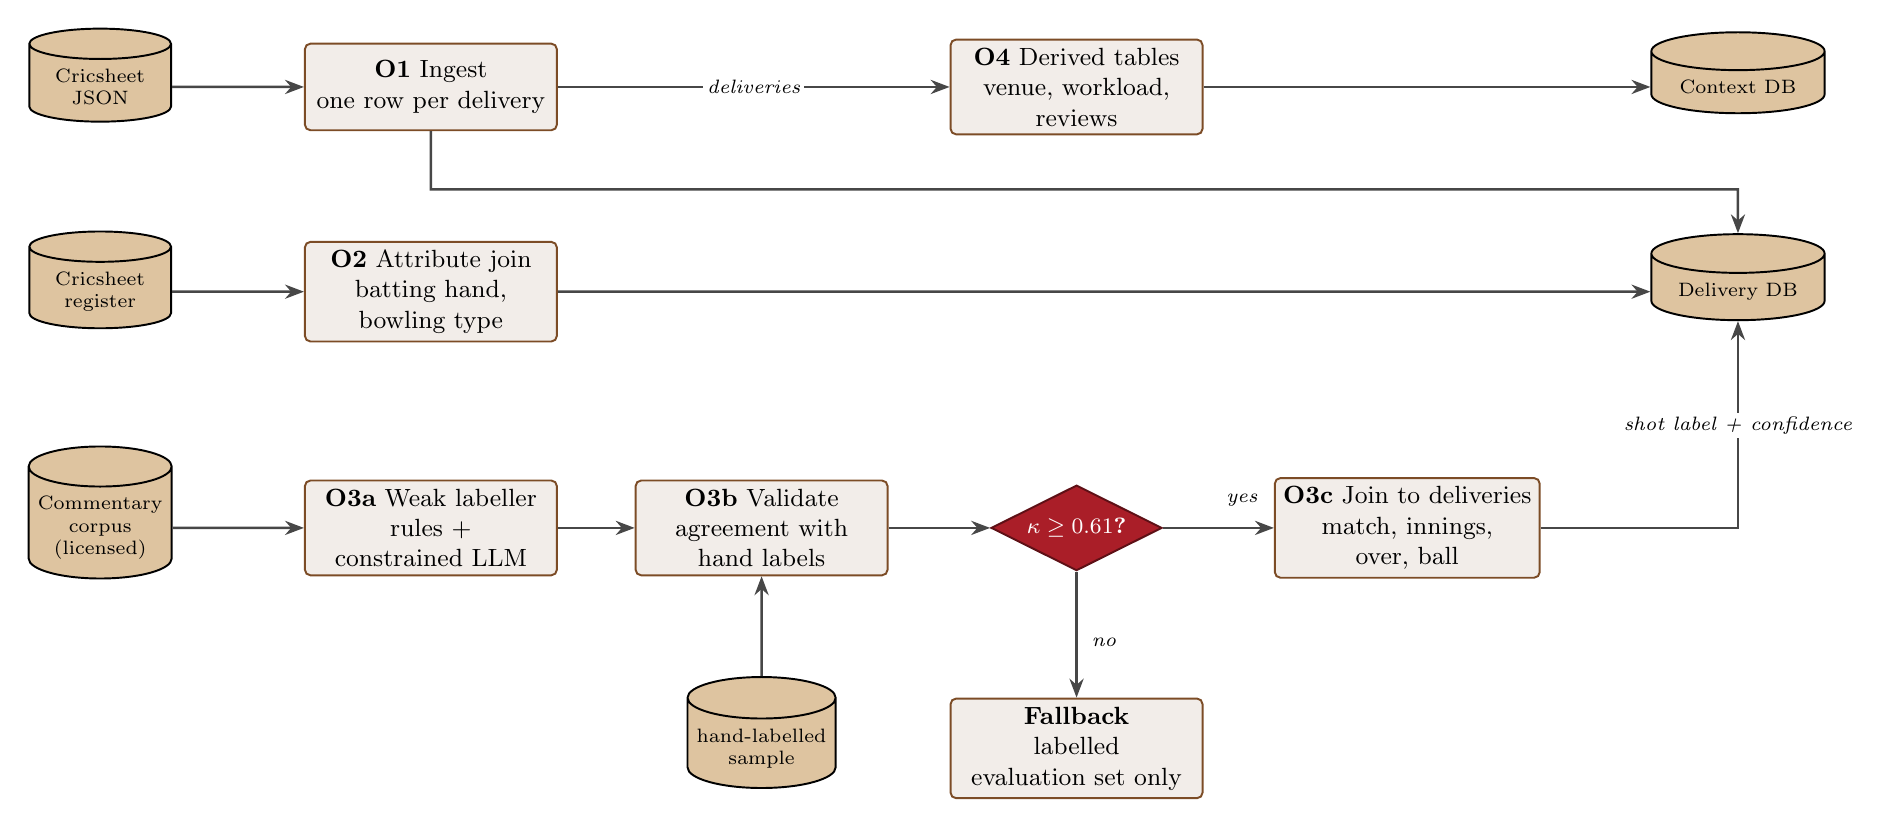
\begin{tikzpicture}

% ---- sources
\node[db] (s1) at (0,0)    {Cricsheet\\JSON};
\node[db] (s2) at (0,-2.6) {Cricsheet\\register};
\node[db] (s3) at (0,-5.6) {Commentary\\corpus\\(licensed)};

% ---- processing
\node[off] (o1)  at (4.2,0)    {\textbf{O1} Ingest\\one row per delivery};
\node[off] (o4)  at (12.4,0)   {\textbf{O4} Derived tables\\venue, workload,\\reviews};
\node[off] (o2)  at (4.2,-2.6) {\textbf{O2} Attribute join\\batting hand,\\bowling type};
\node[off] (o3a) at (4.2,-5.6) {\textbf{O3a} Weak labeller\\rules +\\constrained LLM};
\node[off] (o3b) at (8.4,-5.6) {\textbf{O3b} Validate\\agreement with\\hand labels};
\node[confgate] (kg) at (12.4,-5.6) {$\kappa \geq 0.61$?};
\node[off] (o3c) at (16.6,-5.6) {\textbf{O3c} Join to deliveries\\match, innings,\\over, ball};
\node[db]  (hl)  at (8.4,-8.4) {hand-labelled\\sample};
\node[off] (fb)  at (12.4,-8.4) {\textbf{Fallback}\\labelled\\evaluation set only};

% ---- outputs
\node[db, minimum width=2.2cm] (cdb) at (20.8,0)    {Context DB};
\node[db, minimum width=2.2cm] (ddb) at (20.8,-2.6) {Delivery DB};

% ---- edges
\draw[flow] (s1) -- (o1);
\draw[flow] (s2) -- (o2);
\draw[flow] (s3) -- (o3a);
\draw[flow] (o1) -- (o4);
\node[elab] at (8.3,0) {deliveries};
\draw[flow] (o4) -- (cdb);
\draw[flow] (o1.south) -- (4.2,-1.3) -- (20.8,-1.3) -- (ddb.north);
\draw[flow] (o2) -- (ddb);
\draw[flow] (o3a) -- (o3b);
\draw[flow] (hl) -- (o3b);
\draw[flow] (o3b) -- (kg);
\draw[flow] (kg) -- (o3c);
\node[elab] at (14.5,-5.25) {yes};
\draw[flow] (kg) -- (fb);
\node[elab] at (12.75,-7.05) {no};
\draw[flow] (o3c.east) -- (20.8,-5.6) -- (ddb.south);
\node[elab] at (20.8,-4.3) {shot label + confidence};

\end{tikzpicture}}
\captionof{figure}{Offline evidence pipeline. Nothing here runs at query time.
The commentary bridge (O3) is accepted only if its labels agree substantially
with a hand-labelled sample; otherwise shot-keyed statistics are restricted to a
hand-labelled evaluation set.}
\label{fig:offline}
\end{center}

\paragraph{O1, O2, O4: ball-by-ball evidence.} O1 flattens Cricsheet into one
row per delivery. O2 attaches batting hand and bowling type through the player
register, so that filters such as ``against pace'' have a source. O4 derives the
tables the new N8 modules read: venue aggregates, balls bowled per bowler per
date, and the DRS reviews attached to deliveries.

\paragraph{O3: the commentary-to-shot bridge.} Ball-by-ball commentary names the
stroke (``drives through cover'', ``pulls to deep square''), but no labelled
dataset pairs commentary with the fifteen CricShot10k classes. O3a labels each
line weakly \cite{snorkel}: keyword rules first, and for lines the rules cannot
resolve, a language model whose output is constrained to the fifteen classes or
\emph{none}. O3b measures agreement with a stratified hand-labelled sample of
about 500 lines by Cohen's $\kappa$ \cite{cohen} and per-class F1; the bridge is
accepted at $\kappa \geq 0.61$, ``substantial'' agreement \cite{landis}. O3c joins
labels to deliveries by match, innings, over and ball. Wides and no-balls make
this join error-prone, as Cricsheet's own corrections to its review data show
\cite{cricsheetreview}, so each label carries its confidence and origin (rule or
model). The language model is used offline, to produce categories that are
validated before use; it produces no number an agent can cite, so invariant I1
is untouched.

\paragraph{N7a and N7b.} N7a filters by the full subject tuple from N3 (batter,
bowler, shot, phase, bowler type, venue) and returns the matching deliveries
with their count. A shot filter applies only to deliveries the bridge labelled.
N7b retrieves career and venue context as before.

\subsection{N8 Descriptive Engine (Changes 3 and 4)}

N8 stays deterministic aggregation: every output can be recomputed by hand. It
gains three modules, each of which backs an agent that had no engine before.

\begin{description}[leftmargin=1.2em,style=nextline,itemsep=2pt]
\item[M1 --- delivery statistics.] Strike rate, dismissal rate and sample size
  for any subject tuple, plus differences between two tuples with a bootstrap
  95\% interval (used by check C4).
\item[M2 --- venue profile] (backs N11f). Average first-innings score, share of
  matches won chasing, and the share of wickets taken by pace and by spin.
\item[M3 --- bowling workload] (backs N11k). Balls bowled in the last 7 and 28
  days and their ratio, the acute:chronic workload ratio. Workload spikes were
  associated with roughly double the injury risk in the following week in elite
  fast bowlers \cite{hulin}, but the ratio's validity is disputed
  \cite{impellizzeri}, and match data omits training loads. M3 therefore emits a
  \emph{monitoring flag}, never an injury probability.
\item[M4 --- DRS reviews] (backs N11i). Review counts and overturn rates by team
  and by dismissal type.
\end{description}

\subsection{N9 Predictive Engine and Honest Uncertainty (Changes 2 and 4)}
\label{sec:uncert}

\paragraph{T1 and T2.} Tier~1 is v2's delivery question (``six short balls: what
is the chance of a wicket?''). Tier~2 adds matchup counterfactuals (``what if
this bowler bowled the over instead of that one?''), estimated from head-to-head
rates shrunk toward population rates \cite{efron}. Following the N9 design note,
a counterfactual is always reported as a difference against a baseline, with an
interval; if the interval contains zero, the output is \emph{no detectable
difference}. Tier~3 (batting order, chases) remains future work.

\paragraph{Two kinds of uncertainty.} v2's interval measures only Monte Carlo
error, which shrinks as trials increase. It omits estimation uncertainty, which
shrinks only with more data. The difference is large. On the synthetic corpus
(illustrative only), the batter's pull has 4 dismissals in 50 balls:

\begin{center}
\small
\begin{tabular}{@{}lcc@{}}
\toprule
& \textbf{P(out within 6 balls)} & \textbf{95\% interval} \\
\midrule
v2: Monte Carlo error only (20,000 trials) & 0.394 & [0.387, 0.400] \\
v3: estimation uncertainty propagated & 0.405 (median) & [0.155, 0.697] \\
\bottomrule
\end{tabular}
\end{center}

\noindent The v3 row draws the per-ball rate from a Beta posterior (Jeffreys
prior; shrinkage toward the population would change it again) and pushes each
draw through the simulation. The honest interval is about twenty times wider,
and it spans three wording bands of Table~\ref{tab:lexicon}. v2's interval
would have licensed a confidence the evidence does not support.

\paragraph{Calibration.} T1 and T2 are calibrated on a held-out season:
predicted probabilities against observed frequencies (reliability diagrams) and
the Brier score \cite{brier}. An optional adjustment of rates by measured
posture stays off by default until it is validated, as the N9 design note
requires.

\subsection{N10 Supervisor Router}

The language-model router now receives a short evidence summary: which claim
types are satisfiable for this query (posture only with a clip, matchups only
with two named bowlers, venue claims only with a venue). Fixed rules then apply
a capability filter (an agent with no satisfiable claim type is not woken), the
cap of four active agents, and the default pair. The bounds of v2 are unchanged.

\subsection{The Twelve Stakeholder Agents}

\begin{center}
\footnotesize
\renewcommand{\arraystretch}{1.25}
\begin{tabular}{@{}>{\raggedright\arraybackslash}p{2.5cm}
                  >{\raggedright\arraybackslash}p{2.9cm}
                  >{\raggedright\arraybackslash}p{5.5cm}
                  >{\raggedright\arraybackslash}p{0.9cm}
                  >{\raggedright\arraybackslash}p{3.0cm}@{}}
\toprule
\textbf{Stakeholder} & \textbf{Agent} & \textbf{Claim types it may assert} & \textbf{Prov.} & \textbf{Versus v2} \\
\midrule
Franchises / Boards & Club Operations (N11a) & strike rate, dismissal rate, sample size; venue profile & D & no salary claims without a market engine \\
Coaches & Tactical Analysis (N11b) & strike and dismissal rates; P(dismissal within $k$); matchup difference & D, P & interval now mandatory \\
Players & Personal Performance (N11c) & strike rates; posture metrics & D, M & posture now measured \\
Scouts & Global Scouting (N11d) & strike rate, career strike rate, league benchmark & D & --- \\
Fans & Fan Concierge (N11e) & venue strike rate, strike rate, recent form & D & advice must cite D facts \\
Stadiums / curators & Stadium Operations (N11f) & first-innings average, chasing share, pace and spin wicket share & D & now backed by M2 \\
Bowlers / bowling coaches & \textbf{Bowling Performance (N11g)} & economy and dismissal rate by phase and batting hand; matchup difference & D, P & \textbf{new}; replaces Sponsorship \\
Broadcasters / sponsors & Content Production (N11h) & strike rates; boundary counts as a visibility proxy & D & absorbs Sponsorship \\
Governing bodies / umpires & \textbf{Match Officials (N11i)} & review counts, overturn rate by team and dismissal type & D & \textbf{reframed} from Compliance; backed by M4 \\
Academies & Talent Development (N11j) & strike rates; posture metrics & D, M & posture now measured \\
Medical teams & Injury Management (N11k) & balls bowled (7 and 28 days), workload ratio flag & D & backed by M3; a flag, never a prediction \\
Player agents & Player Representation (N11l) & strike rate, career strike rate & D & no valuation claims without a market engine \\
\bottomrule
\end{tabular}
\captionof{table}{The Version~3 roster. Every claim type in the third column is
a registry entry backed by an engine metric (invariant I2). Adding a market
engine from public auction prices would restore valuation claims for N11a and
N11l: one registry entry and one N8 module, with no change to the graph.}
\label{tab:roster}
\end{center}

\noindent Two agents now cite predictions (N11b, N11g); in v2 only N11b did.
Every current agent reasons about the batter, so N11g fills a real coverage gap;
Cricsheet records the bowler of every delivery.

% =====================================================================
\section{The Claim Contract (Change 1)}

An agent finding is a list of claims and a prose template. The claim is the unit
of verification:

\noindent\begin{minipage}{\textwidth}
{\footnotesize
\begin{verbatim}
{"id": "c1", "kind": "descriptive", "metric": "strike_rate", "engine": "N8.M1",
 "subject": {"player": "Kohli", "shot": "Cover Drive", "phase": "powerplay",
             "bowler_type": "pace"},
 "value": 142.0, "n": 50}
{"id": "c2", "kind": "predictive", "metric": "p_dismissal_within_k", "engine": "N9.T1",
 "subject": {"player": "Kohli", "shot": "Pull", "phase": "powerplay",
             "bowler_type": "pace", "k": 6},
 "value": 0.405, "ci95": [0.155, 0.697], "band": "about even"}

template: "Against pace in the powerplay, Kohli's cover drive returns {c1}.
           Six short balls carry {c2} of a dismissal."
\end{verbatim}}
\end{minipage}

\noindent A deterministic renderer replaces each reference with the verified
value and its provenance tag, for example ``a strike rate of 142.0 [D, 50
balls]''. The agent never types a digit (invariant I3). Findings are produced
under constrained decoding against this schema; a finding that does not parse
fails check C1.

\paragraph{The claim-type registry.} Table~\ref{tab:registry} shows part of the
registry. It is built with the graph, and two things are checked then: every
claim type an agent declares exists, and every registry entry resolves to an
engine metric. A template that asserts ``the surface is holding pace'' with no
venue metric behind it is therefore not a runtime failure but a build failure.

\begin{center}
\footnotesize
\renewcommand{\arraystretch}{1.2}
\begin{tabular}{@{}>{\raggedright\arraybackslash}p{4.3cm}
                  >{\raggedright\arraybackslash}p{1.0cm}
                  >{\raggedright\arraybackslash}p{1.3cm}
                  >{\raggedright\arraybackslash}p{4.2cm}
                  >{\raggedright\arraybackslash}p{4.1cm}@{}}
\toprule
\textbf{Claim type} & \textbf{Prov.} & \textbf{Source} & \textbf{Required subject keys} & \textbf{Checks} \\
\midrule
\texttt{strike\_rate} & D & N8.M1 & player; shot, phase, bowler type optional & C2 exact; C3 floor \\
\texttt{dismissal\_rate} & D & N8.M1 & as above & C2; C3 \\
\texttt{sr\_difference} & D & N8.M1 & player, two shots; phase, bowler type optional & C2; C4 zero-crossing \\
\texttt{venue\_first\_innings\_avg} & D & N8.M2 & venue, format & C2; C3 (matches) \\
\texttt{workload\_ratio\_flag} & D & N8.M3 & bowler, date & C2; wording: flag only \\
\texttt{review\_overturn\_rate} & D & N8.M4 & team or dismissal type & C2; C3 \\
\texttt{weight\_transfer} & M & N6 & clip & C2; video path only \\
\texttt{p\_dismissal\_within\_k} & P & N9.T1 & player, shot, phase, bowler type, $k$ & C2 with interval; C4 band \\
\texttt{matchup\_difference} & P & N9.T2 & batter, two bowlers, phase, $k$ & C2 with interval; C4 zero-crossing \\
\bottomrule
\end{tabular}
\captionof{table}{Part of the claim-type registry.}
\label{tab:registry}
\end{center}

% =====================================================================
\section{Faith Check v3}
\label{sec:faith}

\begin{center}
\resizebox{\textwidth}{!}{%
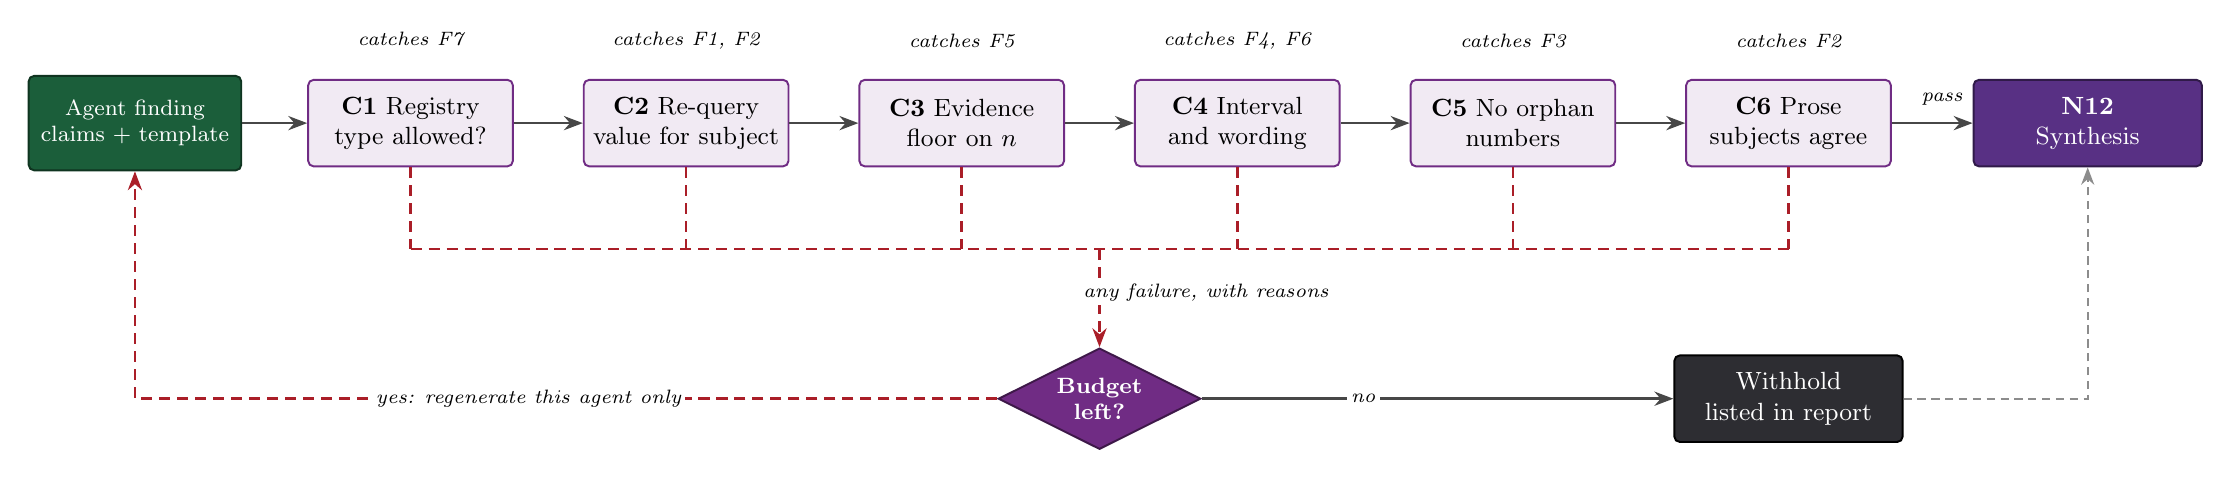
\begin{tikzpicture}

\node[agent] (fd) at (0,0)    {Agent finding\\claims + template};
\node[chk] (c1) at (3.5,0)  {\textbf{C1} Registry\\type allowed?};
\node[chk] (c2) at (7.0,0)  {\textbf{C2} Re-query\\value for subject};
\node[chk] (c3) at (10.5,0) {\textbf{C3} Evidence\\floor on $n$};
\node[chk] (c4) at (14.0,0) {\textbf{C4} Interval\\and wording};
\node[chk] (c5) at (17.5,0) {\textbf{C5} No orphan\\numbers};
\node[chk] (c6) at (21.0,0) {\textbf{C6} Prose\\subjects agree};
\node[route] (s12) at (24.8,0) {\textbf{N12}\\Synthesis};

\node[elab] at (3.5,1.05)  {catches F7};
\node[elab] at (7.0,1.05)  {catches F1, F2};
\node[elab] at (10.5,1.05) {catches F5};
\node[elab] at (14.0,1.05) {catches F4, F6};
\node[elab] at (17.5,1.05) {catches F3};
\node[elab] at (21.0,1.05) {catches F2};

\draw[flow] (fd) -- (c1);
\draw[flow] (c1) -- (c2);
\draw[flow] (c2) -- (c3);
\draw[flow] (c3) -- (c4);
\draw[flow] (c4) -- (c5);
\draw[flow] (c5) -- (c6);
\draw[flow] (c6) -- (s12);
\node[elab] at (22.95,0.3) {pass};

\draw[redbus] (c1.south) -- (3.5,-1.6);
\draw[redbus] (c2.south) -- (7.0,-1.6);
\draw[redbus] (c3.south) -- (10.5,-1.6);
\draw[redbus] (c4.south) -- (14.0,-1.6);
\draw[redbus] (c5.south) -- (17.5,-1.6);
\draw[redbus] (c6.south) -- (21.0,-1.6);
\draw[redbus] (3.5,-1.6) -- (21.0,-1.6);

\node[faithgate] (rg) at (12.25,-3.5) {Budget\\left?};
\draw[redloop] (12.25,-1.6) -- (rg.north);
\node[elab] at (13.6,-2.15) {any failure, with reasons};
\draw[redloop] (rg.west) -- (0,-3.5) -- (fd.south);
\node[elab] at (5.0,-3.5) {yes: regenerate this agent only};
\node[outnode] (wh) at (21.0,-3.5) {Withhold\\listed in report};
\draw[flow] (rg.east) -- (wh.west);
\node[elab] at (15.6,-3.5) {no};
\draw[withhold] (wh.east) -- (24.8,-3.5) -- (s12.south);

\end{tikzpicture}}
\captionof{figure}{Faith Check v3. The six checks run in order, cheapest first,
inside the single Faith Check node. Each catches particular fabrication classes
of Table~\ref{tab:fab}.}
\label{fig:faith-v3}
\end{center}

\begin{description}[leftmargin=1.2em,style=nextline,itemsep=2pt]
\item[C1 --- Schema and registry.] The finding parses; each claim type exists
  and this agent is allowed to assert it; the claim names its source.
\item[C2 --- Subject-bound value.] The gate re-queries the named source with the
  claim's subject tuple and compares the result within rounding, including the
  interval for predictive claims. A correct number cited for the wrong subject
  fails here, because the engine returns a different value for that subject.
\item[C3 --- Evidence floor.] A descriptive claim on fewer than $n_{\min}$ balls
  (a design parameter; default 30) must carry a small-sample qualifier, and may
  not be generalised (``struggles against spin'') without one.
\item[C4 --- Interval and wording.] A predictive claim's wording must fall in
  the band of Table~\ref{tab:lexicon} that contains its point estimate; if the
  interval crosses a band boundary, a hedge naming the evidence is required. A
  comparative claim, predictive or descriptive, whose difference interval
  contains zero must say \emph{no detectable difference}.
\item[C5 --- No orphan numbers.] Apart from claim references and a small
  allowlist (``T20'', ``U-19''), the template contains no digits. This closes
  the uncited-figure gap of v2 by construction.
\item[C6 --- Prose subjects agree.] Using a gazetteer built from the player
  register, the fifteen shot names and their synonyms, phases, bowler types and
  venues, every entity named in a sentence that contains a claim reference must
  agree with that claim's subject.
\end{description}

\paragraph{Worked example: the v2 running example.} On the synthetic corpus the
batter's cover drive returns a strike rate of 142.0 and his pull 112.0, both on
50 balls. The bootstrap 95\% interval for the difference is $[-16.0,\ +76.0]$,
which contains zero. Under C4, the v2 template's verdict that the cover drive
is ``the stronger stroke'' is a spurious difference (class F6): the agent must
report no detectable difference on this evidence. The example is illustrative,
but it shows that the stricter gate changes conclusions, not only formatting.

\begin{center}
\footnotesize
\renewcommand{\arraystretch}{1.2}
\begin{tabular}{@{}>{\raggedright\arraybackslash}p{3.2cm}
                  >{\raggedright\arraybackslash}p{5.4cm}
                  >{\raggedright\arraybackslash}p{5.6cm}@{}}
\toprule
\textbf{Point estimate $p$} & \textbf{Required wording (any of)} & \textbf{Forbidden in this band} \\
\midrule
$p \leq 0.13$ & almost certainly not, remote & likely, probable, possible \\
$0.13 < p \leq 0.40$ & probably not, unlikely & likely, probable, expected \\
$0.40 < p < 0.60$ & about even, as likely as not & likely, unlikely \\
$0.60 \leq p < 0.87$ & probable, likely & almost certain, will \\
$p \geq 0.87$ & almost certain, very likely & certain, guaranteed \\
any band & --- & will, certain, guaranteed, always, never \\
\bottomrule
\end{tabular}
\captionof{table}{Wording bands for predictive claims, after Kent's words of
estimative probability \cite{kent}, with his ranges closed into contiguous
intervals. If the 95\% interval crosses a boundary, a hedge naming the evidence
(``on 4 dismissals in 50 balls'') is also required.}
\label{tab:lexicon}
\end{center}

\noindent On the Tier~1 example of Section~\ref{sec:uncert}, the median of 0.405
falls in \emph{about even} and the interval crosses two boundaries, so an
acceptable rendering is ``about as likely as not, though on 4 dismissals in 50
balls the estimate is very uncertain''. ``Will probably get him out'' fails C4.

\paragraph{N12 and N13.} N12 composes the report from verified findings only and
is held to the same rule: it references claims and types no numbers, and its
output passes C5 and C6. If it fails, the report falls back to the verified
findings in fixed order, which keeps the step bounded. N13 shows every number
with its provenance tag and lists withheld findings.

% =====================================================================
\section{Control Loops and Bounds}

The two loops of v2 are unchanged in structure. The retry loop guards against
perception errors; the regenerate loop now re-runs only the failing agents and
passes them the failing checks and reasons. Agent invocations remain bounded by
$4 \times (1 + 2) = 12$, independent of roster size. N2b runs in parallel with
the N2--N5 chain, and checks C1--C6 run inside the single Faith Check node, so
the superstep bound of v2 is expected to hold; it must be re-derived from the
closed-form cost model and re-measured before it is claimed.

% =====================================================================
\section{Evaluation Plan}

\paragraph{Fabrication containment.} The existing injection harness is extended
from three fabrication classes to seven (Table~\ref{tab:fab}). The v2 column
follows from the v2 code, which compares cited values only; it is a prediction
to be confirmed, not a measurement. Each class is measured by catch rate, and
correct findings by false-rejection rate, regeneration count and report
completeness.

\begin{center}
\footnotesize
\renewcommand{\arraystretch}{1.2}
\begin{tabular}{@{}>{\raggedright\arraybackslash}p{1.0cm}
                  >{\raggedright\arraybackslash}p{3.2cm}
                  >{\raggedright\arraybackslash}p{5.2cm}
                  >{\raggedright\arraybackslash}p{2.0cm}
                  >{\raggedright\arraybackslash}p{2.2cm}@{}}
\toprule
\textbf{Class} & \textbf{Injected error} & \textbf{Example} & \textbf{v2 gate} & \textbf{v3 check} \\
\midrule
F1 & wrong value & strike rate 162 instead of 142 & caught & C2 \\
F2 & right value, wrong subject & one batter's 142 attributed to another & missed & C2, C6 \\
F3 & uncited number & ``about 150'' typed in the prose & missed & C5 \\
F4 & certainty inflation & ``will likely be dismissed'' at $p = 0.405$ & missed & C4 \\
F5 & small-sample generalisation & ``struggles against spin'' on six balls & missed & C3 \\
F6 & spurious difference & ``the stronger stroke'' when the interval contains zero & missed & C4 \\
F7 & unsupported claim type & ``the surface is holding pace'' with no venue metric & missed & C1, registry \\
\bottomrule
\end{tabular}
\captionof{table}{Fabrication classes for the injection harness.}
\label{tab:fab}
\end{center}

\paragraph{Engines and evidence.} N8 modules are checked by recomputation
against hand-computed cases. N9 T1 and T2 are checked for calibration on a
held-out season. The commentary bridge reports $\kappa$ and per-class F1 against
hand labels. Posture reports the front-foot versus back-foot AUC of each metric.

\paragraph{Routing and cost.} The labelled routing set is extended with queries
for N11g and N11i, since every added role is a new way for the router to be
wrong. The cost model's bounds are re-derived for the v3 graph before they are
measured.

% =====================================================================
\section{Build Plan}

\begin{center}
\footnotesize
\renewcommand{\arraystretch}{1.2}
\begin{tabular}{@{}>{\raggedright\arraybackslash}p{2.6cm}
                  >{\raggedright\arraybackslash}p{7.4cm}
                  >{\raggedright\arraybackslash}p{1.4cm}
                  >{\raggedright\arraybackslash}p{3.2cm}@{}}
\toprule
\textbf{Phase} & \textbf{Work} & \textbf{Days} & \textbf{Depends on} \\
\midrule
1 Contract & claim schema, renderer, registry; checks C1, C2, C5, C6 & 3--5 & --- \\
1 Contract & wording bands; checks C3, C4; N9 intervals with estimation uncertainty & 3--4 & --- \\
2 Honest agents & N8 modules M2--M4; roster changes including N11g & 3--5 & phase 1 \\
3 Real evidence & O1, O2, O4; M1 on Cricsheet data & 3--4 & --- \\
3 Real evidence & N9 Tier~2 with calibration on a held-out season & 4--5 & O1, O2 \\
Evaluation & fabrication classes F1--F7; v2 against v3 & 2 & phases 1--2 \\
\midrule
\textbf{Core total} & & \textbf{18--25} & \\
\midrule
4 Optional & commentary bridge O3, with validation & 10--15 & O1; a licensed corpus \\
4 Optional & N2b pose estimator and posture validation & 3--5 & --- \\
\bottomrule
\end{tabular}
\captionof{table}{Build plan. Estimates, not commitments. Phase~1 replaces the
1--2 day structured-citation block of the completion estimate, and phase~3
replaces its 2--3 day data-layer block.}
\label{tab:build}
\end{center}

% =====================================================================
\section{Risks and Fallbacks}

\begin{center}
\footnotesize
\renewcommand{\arraystretch}{1.2}
\begin{tabular}{@{}>{\raggedright\arraybackslash}p{4.6cm}
                  >{\raggedright\arraybackslash}p{4.0cm}
                  >{\raggedright\arraybackslash}p{6.0cm}@{}}
\toprule
\textbf{Risk} & \textbf{Effect} & \textbf{Fallback} \\
\midrule
No licensed commentary corpus with match and ball keys & O3 impossible & hand-label an evaluation set; shot-keyed claims only on it \\
Bridge labels too noisy ($\kappa < 0.61$) & wrong shot statistics & disable the shot filter on real data; report the bridge as a negative result \\
A 7B model breaks the claim schema & findings do not parse & constrained decoding; parse failures count as C1 rejections and regenerate \\
Pose fails on low-resolution clips & no posture & metrics failing validation leave the registry; agents degrade to D claims \\
Workload ratio validity disputed & misleading medical advice & worded as a monitoring flag; never a probability \\
Bowling type missing for some players & filters silently shrink $n$ & $n$ is always reported; C3 floor \\
New roles confuse the router & wrong agents woken & larger labelled routing set; capability filter \\
\bottomrule
\end{tabular}
\captionof{table}{Risks and fallbacks.}
\label{tab:risks}
\end{center}

% =====================================================================
\section{Positioning against Related Work}

Verifying a language model's numbers against a trusted source is an active
area. Proof-Carrying Numbers \cite{pcn} requires each displayed number to link
to a verified structured claim or be marked unverified. Tool receipts
\cite{receipts} check an agent's claims against signed records of the tool calls
it actually made. Work on collective hallucination \cite{collective} decomposes
multi-agent outputs into atomic claims. CricketMind v2 belongs to this family,
and v3 must be presented against it. Three elements of v3 are, as far as a
limited search found, not covered there:

\begin{enumerate}[nosep,leftmargin=1.6em]
\item \textbf{Subject binding.} Claims are tuples re-queried against the engine
  for their subject (C2), and the prose's named entities must agree with them
  (C6).
\item \textbf{Uncertainty faithfulness.} The wording of predictive and
  comparative claims is checked against an \emph{external} engine's interval,
  one that includes estimation uncertainty (C4). Research on verbalised
  confidence \cite{lin2022, wang2024} studies how well a model states its
  \emph{own} confidence, which is a different question.
\item \textbf{A static registry of claim types} that refuses, at build time,
  kinds of claims that no engine computes (I2).
\end{enumerate}

\noindent In cricket, FanCric \cite{fancric} coordinates language-model agents
for fantasy team selection. CricBench \cite{cricbench} found that most SQL
generated by language models for cricket analytics questions executes, while
far less is semantically correct: direct evidence for the premise that cricket
numbers produced by language models must be verified. Before any novelty claim
is submitted, this positioning needs a systematic literature search.

% =====================================================================
\section{What This Document Does Not Claim}

\begin{itemize}[nosep,leftmargin=1.6em]
\item No v3 component has been built, and no v3 result has been measured.
\item The worked examples use the synthetic corpus and say nothing about real
  players.
\item The perception front end's accuracy is outside the scope of this document.
\item The workload flag is not an injury predictor.
\item Shot-keyed statistics on real data exist only if the commentary bridge
  passes validation.
\end{itemize}

% =====================================================================
\begin{thebibliography}{99}
\small

\bibitem{cricshot10k}
M. K. Dihan, Abdullah, Amina, and S. Ahmed, ``CricShot10k: A large-scale video
dataset for cricket shot classification,'' \emph{IEEE Access}, 2026,
doi:10.1109/ACCESS.2026.3663220.

\bibitem{cricsheet}
S. Rushe, ``Cricsheet: Freely-available structured data for cricket,''
\url{https://cricsheet.org}.

\bibitem{cricsheetreview}
S. Rushe, ``Review corrections,'' Cricsheet,
\url{https://cricsheet.org/article/review_corrections/}.

\bibitem{cricketdata}
R. J. Hyndman \emph{et al.}, ``cricketdata: International cricket data,'' R
package, \url{https://pkg.robjhyndman.com/cricketdata/}.

\bibitem{yolo}
G. Jocher, A. Chaurasia, and J. Qiu, ``Ultralytics YOLO,'' 2023,
\url{https://github.com/ultralytics/ultralytics}.

\bibitem{snorkel}
A. Ratner, S. H. Bach, H. Ehrenberg, J. Fries, S. Wu, and C. R\'e, ``Snorkel:
Rapid training data creation with weak supervision,'' \emph{Proc. VLDB
Endowment}, vol.~11, no.~3, pp.~269--282, 2017.

\bibitem{cohen}
J. Cohen, ``A coefficient of agreement for nominal scales,'' \emph{Educational
and Psychological Measurement}, vol.~20, no.~1, pp.~37--46, 1960.

\bibitem{landis}
J. R. Landis and G. G. Koch, ``The measurement of observer agreement for
categorical data,'' \emph{Biometrics}, vol.~33, no.~1, pp.~159--174, 1977.

\bibitem{hulin}
B. T. Hulin, T. J. Gabbett, P. Blanch, P. Chapman, D. Bailey, and J. W.
Orchard, ``Spikes in acute workload are associated with increased injury risk
in elite cricket fast bowlers,'' \emph{British Journal of Sports Medicine},
vol.~48, no.~8, pp.~708--712, 2014.

\bibitem{impellizzeri}
F. M. Impellizzeri, S. Woodcock, A. J. Coutts, M. Fanchini, A. McCall, and
A. D. Vigotsky, ``What role do chronic workloads play in the acute to chronic
workload ratio? Time to dismiss ACWR and its underlying theory,''
\emph{Sports Medicine}, vol.~51, no.~3, pp.~581--592, 2021.

\bibitem{efron}
B. Efron and C. Morris, ``Data analysis using Stein's estimator and its
generalizations,'' \emph{Journal of the American Statistical Association},
vol.~70, no.~350, pp.~311--319, 1975.

\bibitem{brier}
G. W. Brier, ``Verification of forecasts expressed in terms of probability,''
\emph{Monthly Weather Review}, vol.~78, no.~1, pp.~1--3, 1950.

\bibitem{kent}
S. Kent, ``Words of estimative probability,'' \emph{Studies in Intelligence},
vol.~8, no.~4, pp.~49--65, 1964.

\bibitem{pcn}
A. V. Solatorio, ``Proof-Carrying Numbers (PCN): A protocol for trustworthy
numeric answers from LLMs via claim verification,'' arXiv:2509.06902, 2025.

\bibitem{receipts}
A. Basu, ``Tool receipts, not zero-knowledge proofs: Practical hallucination
detection for AI agents,'' arXiv:2603.10060, 2026.

\bibitem{collective}
S. Jamshidi, ``Collective hallucination in multi-agent LLMs: Modeling and
defense,'' arXiv:2606.07941, 2026.

\bibitem{lin2022}
S. Lin, J. Hilton, and O. Evans, ``Teaching models to express their
uncertainty in words,'' \emph{Transactions on Machine Learning Research}, 2022,
arXiv:2205.14334.

\bibitem{wang2024}
C. Wang, G. Szarvas, G. Balazs, P. Danchenko, and P. Ernst, ``Calibrating
verbalized probabilities for large language models,'' arXiv:2410.06707, 2024.

\bibitem{fancric}
M. Bhatnagar, ``FanCric: Multi-agentic framework for crafting fantasy 11
cricket teams,'' arXiv:2410.01307, 2024.

\bibitem{cricbench}
V. Devraj, D. Kumar, and J. S. Challa, ``CricBench: A multilingual benchmark
for evaluating LLMs in cricket analytics,'' arXiv:2512.21877, 2025.

\end{thebibliography}

\end{document}
